\chapter{Аудио Дипфейк}

Под терменом дипфейковым звуком обычно понимается любой звук, важные атрибуты которого были изменены с помощью технологий нейронной сети, но при этом сохраняется его воспринимаемая естественность. Предыдущие исследования в основном включали пять видов дипфейкового звука:

\begin{enumerate}
    \item преобразование текста в речь;
    \item преобразование голоса; 
    \item подделка эмоций;
    \item подделка сцен;
    \item частично подделка.
\end{enumerate}

также в таблице (\ref{table::audio-class}), проведено классификация аудио дипфейков по способу генерации.

\section{Преобразование текста в речь}

Преобразование текста в речь (TTS) [8], широко известное, направлено на синтез понятной и естественной речи, заданной любым произвольным текстом, с использованием моделей, основанных на машинном обучении. Модели TTS могут генерировать реалистичную и похожую на человеческую речь с развитием глубоких нейронных сетей [1]. Системы TTS в основном включают в себя модули анализа текста и генерации речевых сигналов. Существует два основных метода генерации речевых сигналов [13]: 

\begin{itemize}
    \item конкатенативный;
    \item статистический параметрический TTS.
\end{itemize}

\section{Преобразование голоса} 

Преобразование голоса (VC) [8] относится к клонированию голоса человека в цифровом виде. Она направлена на то, чтобы изменить тембр и просодию речи данного говорящего на тембр речи другого говорящего, в то время как содержание речи остается прежним. Вводом в систему VC является естественное высказывание данного говорящего. Существует примерно три основных подхода к технологиям VC [18]: статистический параметрический, частотное искажение и выбор единиц измерения. Статистическая параметрическая модель также имеет вокодер, который аналогичен таковому в статистических параметрических TTS [22].

\section{Подделка эмоций}

Подделка эмоций [25] направлена на изменение звука таким образом, что меняется эмоция речи, в то время как другая информация остается прежней, например, личность говорящего и содержание речи. Изменение эмоций голоса часто приводит к изменению семантики.

\section{Подделка сцен}

Подделка сцены [27] включает в себя сопоставление акустической сцены исходного высказывания с другой сценой с помощью технологий улучшения речи, при этом личность говорящего и содержание речи остаются неизменными.

\section{Частично подделка}

частично подделка [28] фокусируется на изменении лишь нескольких слов в высказывании. Фальшивое высказывание создается путем манипулирования исходными высказываниями с помощью подлинных или синтезированных аудиоклипов. Спикер оригинального высказывания и фейковых клипов — один и тот же человек. Синтезированные аудиоклипы, сохраняя при этом личность говорящего неизменной.

\begin{table}[H]
	\centering
	\setlength{\tabcolsep}{8pt} % Adjust column spacing
	\renewcommand{\arraystretch}{1.3} % Adjust row spacing
    \caption{Класификации аудио дипфейков по способу генерации}\label{tab:class}
    \captionsetup{justification=raggedright,singlelinecheck=false}
    \begin{tabular}{|p{3cm}|p{3cm}| p{3cm}| p{3cm}|}		
        \hline
		Поддельный тип & Поддельная черта & Поддельная продолжительность  & С помощью нейронной сети  \\ 
		\hline
		Преобразование  текста в речь    & Личность спикера, Речевое содержание  & полностью	  	 &  да  \\
		\hline
		Преобразование голоса   & Личность спикера & полностью  &  да \\
		\hline
		Подделка эмоций & эмоция спикера 	& полностью  &  да \\
		\hline
		Подделка сцен  & Акустическая сцена & полностью  &  да \\
		\hline
		Частично подделка  & Речевое содержание 	& частично  &  да \\
		\hline
    \end{tabular}
    \label{table::audio-class}
\end{table}

\chapter{Отличительные признаки аудио для изучения}

Извлечение признаков является ключевым модулем классификатора аудио дипфейков. Целью извлечения признаков является изучение отличительных признаков путем выделения звуковых поддельных артефактов из речевых сигналов. Большое количество усилий показало важность полезных функций для обнаружения поддельных атак. Признаки, использованные в исследованиях, можно условно разделить на четыре категории [48]: 
\begin{itemize}
    \item спектральные особенности;
    \item просодические особенности;
    \item глубокие особенности.
\end{itemize}

\section{спектральные особенности}

Спектральные характеристики в анализе звука относятся к характеристикам, которые показывают распределение энергии по различным частотам в сигнале, эти спектральные характеристики вычисляются с помощью математических преобразований, таких как быстрое преобразование Фурье (FFT), и имеют решающее значение для извлечения значимой информации из аудиосигналов для различных применений, спектральные характеристики могут быть классифицированы на краткосрочные и долгосрочные в зависимости от масштаба времени, в течение которого они вычисляются.

\subsection{Кратковременные спектральные особенности}

Кратковременные спектральные характеристики, извлеченные из коротких кадров, обычно длительностью 20-30 мс, описывают кратковременную спектральную огибающую, включающую акустический коррелят тембра голоса. Кратковременные спектральные характеристики вычисляются главным образом путем применения кратковременного преобразования Фурье (STFT) к речевому сигналу [52]. Учитывая речевой сигнал x(t), предполагается, что он квазистационарен в течение короткого периода. STFT речевого сигнала x(t) формулируется следующим образом:

\begin{equation}
    X(t, \omega) = |X(t, \omega)| e^{j\phi(\omega)}
\end{equation}

где \(|X(t, \omega)|\), это спектр магнитуд а \(\phi(\omega)\) представляет собой фазовый спектр в кадре t и частотный диапазон \(\omega\). Спектр мощности определяется как \(|X(t, \omega)|^2\).

Кратковременные спектральные характеристики в основном состоят из кратковременных характеристик, основанных на магнитуде и фазе. Обычно несколько характеристик, основанных на магнитуде, непосредственно выводятся из спектра магнитуд, но большинство из них выводятся из спектра мощности. Характеристики, основанные на фазе, выводятся из фазового спектра.

\subsection{Долгосрочные спектральные особенности}

Кратковременные спектральные признаки не очень хорошо улавливают временные характеристики траекторий речевых признаков из-за того, что они вычисляются покадрово [60]. Поэтому были предложены долгосрочные спектральные характеристики для получения информации на большом расстоянии из речевых сигналов, и исследования показали, что они имеют решающее значение для обнаружения поддельной речи [49].


\section{Просодические особенности}

Просодия относится к несегментарной информации речевых сигналов, включая ударение на слоге, интонационные паттерны, темп речи и ритм [78]. В отличие от кратковременных спектральных характеристик с короткой продолжительностью, обычно составляющей 20-30 мс, они охватывают более длинные сегменты, такие как телефоны, слоги, слова, высказывания и т.д. Важные просодические параметры включают основную частоту (F0), длительность, распределение энергии, скорость разговора и т.д. Предыдущие исследования [78] по обнаружению поддельного звука в основном рассматривали три основные просодические характеристики:

\begin{itemize}
    \item F0;
    \item продолжительность;
    \item энергию.
\end{itemize}

Эти функции менее чувствительны к канальным эффектам по сравнению со спектральными функциями [8]. Они могут предоставлять дополнительную информацию к спектральным функциям для повышения эффективности обнаружения поддельного звука.

\section{Глубокие возможности}

Вышеупомянутые спектральные особенности и просодические особенности - это почти все функции, созданные вручную, обладающие сильными и желательными репрезентативными способностями. Однако их дизайн испорчен предубеждениями из-за ограничений представлений ручной работы [51]. Таким образом, глубокие функции мотивированы заполнить пробел. Глубокие функции изучаются с помощью глубоких нейронных сетей, которые можно условно разделить на: обучаемые спектральные функции, контролируемые функции встраивания и самоконтролируемые функции встраивания.

На рисунке (\ref{fig:audio-classification}) представлено, класификации аудио по признаками для обучение: 
\begin{figure}[H]
	\centering
	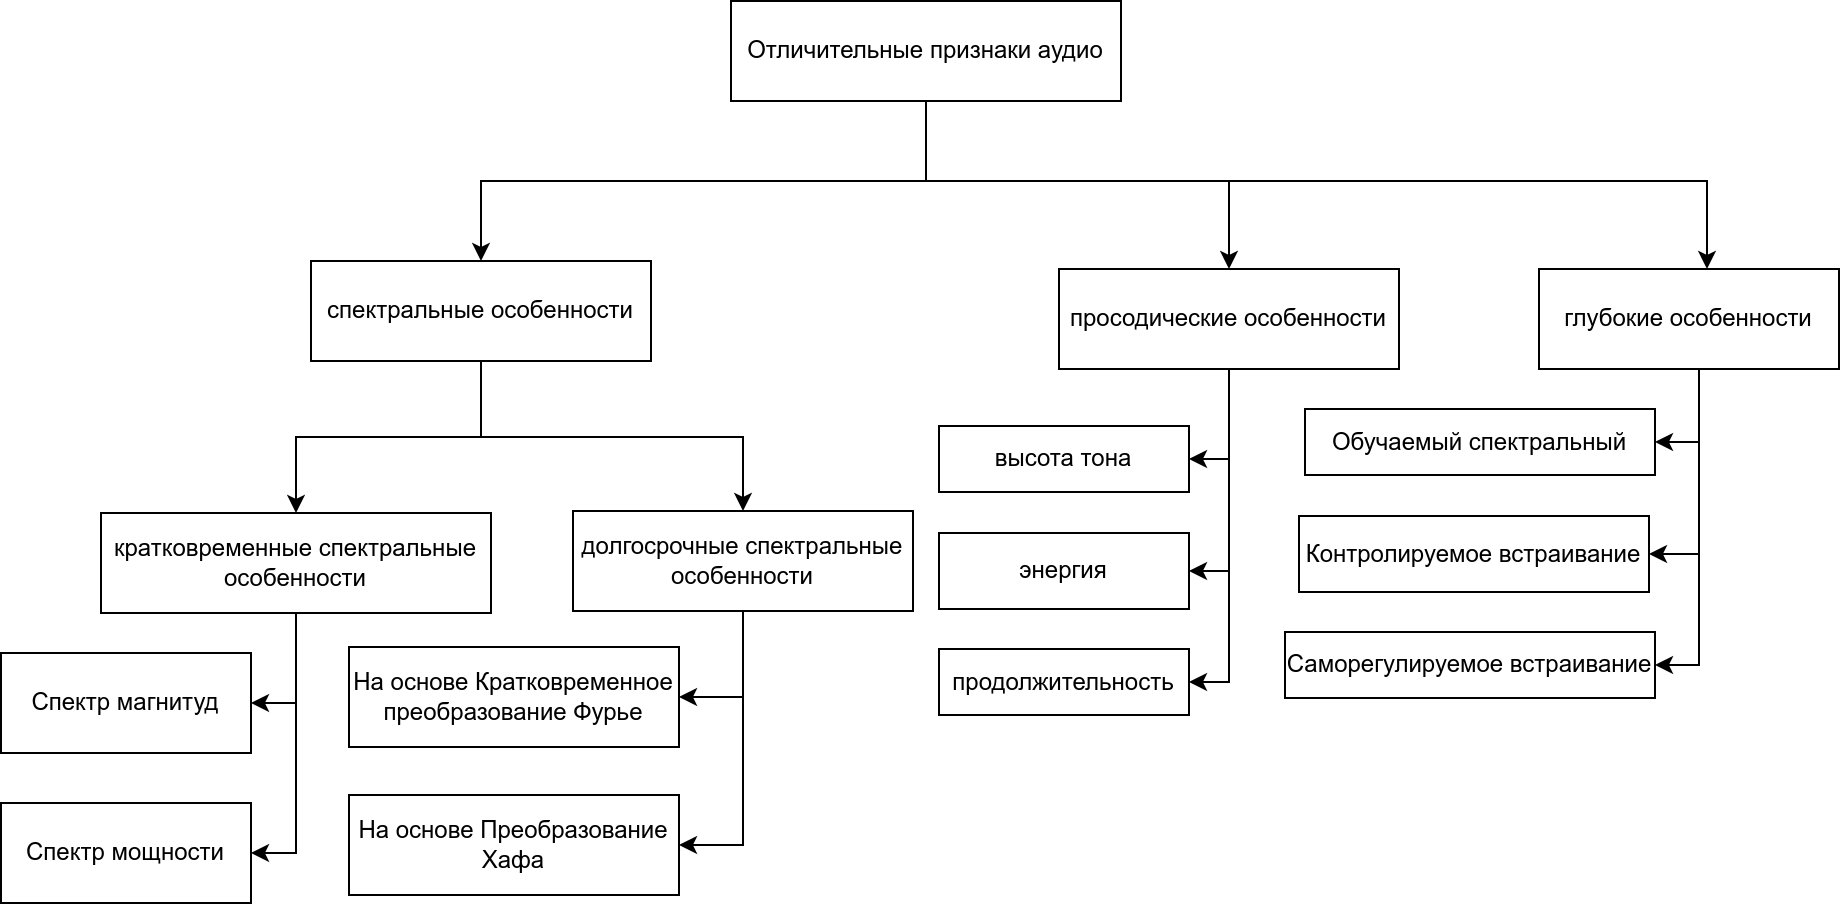
\includegraphics[width=0.9\linewidth]{images/classification-of-audio.png}
	\caption{Классификации аудио по признаками}
	\label{fig:audio-classification}
\end{figure}


\chapter{Методы обнаружения поддельного звука (Аудио Дипфейк)}

В системах, которые изпользуются для обнаружения поддельного звука, важнешей фактором является особенности аудио для изучения и внутренний классификатор очень важен для глубокого распознавания аудио, целью которого является изучение высокоуровневого представления функций входного интерфейса и моделирование превосходных возможностей обнаружения. Внутренний классификатор которые часто используются для обнаружения аудио дипфейков в основном делятся на две категории: 

\begin{itemize}
    \item Статистические методы;
    \item С применением глубоких нейронных сетей.
\end{itemize}

\section{Статистические методы обнаружения Аудио Дипфейк}

Под терменом статистические методы в статей пишут алгоритмы машиное обучение, алгоритмы машиное обучение изучают характеристики аудио и для решение задачой обнаружения аудио дипфейк, используется алгоритмы бинарное классификации.
В связм с этим, для обнаружения фальшивой речи было использовано множество классических подходов к классификации паттернов.
Самые популярные методы обнаружения аудио дипфейк с применением машиное обучение являются:

\begin{itemize}
    \item Машина опорных векторов (SVM);
    \item Гауссовые моделей смеси (GMM).
\end{itemize}

\subsection{Машина опорных векторов (SVM)}

SVM - это контролируемый метод обучения, который основывается в основном на двух предположениях \cite{hamza2022deepfake}:
\begin{enumerate}
    \item Преобразование данных в многомерное пространство может свести сложные проблемы классификации со сложными поверхностями принятия решений к более мелким проблемам, которые могут быть решены путем их линейного разделения;
    \item Только обучающие шаблоны вблизи поверхности принятия решений обеспечивают наиболее чувствительную детали для классификации.
\end{enumerate}

Так как, проблема обнаружения аудио дипфейков представляет собой бинарную классификацию с линейно разделяемыми векторами \(x_{i} \in \mathbb{R}^{n}\), в качестве поверхности принятия решения, используемой для классификации паттерна как принадлежащего к одному из двух классов, используется гиперплоскость \(H_{0}\). Если х это случайный вектор n * \(\mathbb{R}\), тогда мы определяем:

\begin{equation}
    f_{(x)} = w.x + b
\end{equation}

В формуле (.) это скалярное произведение, набор всех x-векторов, удовлетворяющих уравнению \(f_{(x)} = 0\), обозначается как \(H_{0}\). Предполагая две гиперплоскости, H1 и H2, расстояние между ними называется их границей, которую можно представить следующим образом:

\begin{equation}
    \begin{cases}
        H_{1} = \{x \in \mathbb{R}^{n} | f_{(x)} > 0\} \\
        H_{2} = \{x \in \mathbb{R}^{n} | f_{(x)} < 0\}
    \end{cases}
\end{equation}

Гиперплоскость решения H0 зависит от векторов, ближайших к двум параллельным гиперплоскостям, называемым опорными векторами. Запас должен быть максимальным, чтобы получить классификатор, который не очень адаптирован к обучающим данным.

На рисунке (\ref{fig:support-vector-machine}) представлено, машина опорных векторов: 
\begin{figure}[H]
	\centering
	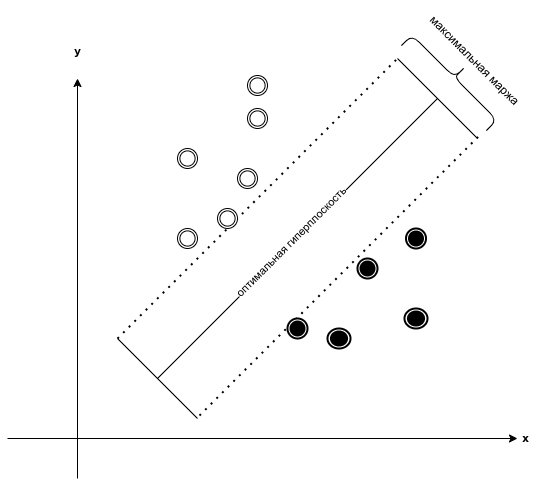
\includegraphics[width=0.4\linewidth]{images/support-vector-machine.png}
	\caption{Машина опорных векторов (SVM)}
	\label{fig:support-vector-machine}
\end{figure}

В многих статей по класификации аудио дипфейков используется метод SVM, который помогает классифицировать аудиосигналы дипфейк. Он хорошо работает с четким разделением выборок и эффективен в средах с высокой размерностью. Он использует подмножество точек обучения в функции принятия решения, что делает его эффективным с точки зрения памяти.

\subsubsection*{Методы с применением SVM}

В статей [110] и [68], используют машина опорных векторов в качестве классификатора, в статей [110] предполагают, что классификаторы SVM по своей сути устойчивы к атакам с искусственным подменой сигналов. Однако очень трудно определить точную природу атак с подменой в практических сценариях.
В статей [68] предложили одноклассовый классификатор SVM, обученный только использованию подлинных высказываний для классификации реальных и поддельных голосов, который хорошо подходит для неизвестных атак с использованием подделки.

\subsection{Гауссовые моделей смеси (GMM)}

Модель гауссовой смеси (GMM), как следует из названия, представляет собой смесь нескольких гауссовых распределений. Речевые признаки представлены в виде векторов в n-мерном пространстве. Распределение этих векторов признаков представлено смесью гауссовых плотностей. \\ Для n-мерного вектора признаков x функция плотности смеси для класса s с параметром модели \(\lambda^{s}\) определяется как \cite{JOTHILAKSHMI2016301}:

\begin{equation}
    p(x | \lambda^{s}) = \sum_{i = 1}^{\mathcal{M}} \alpha^{s}_{i} f_{i}^{s}(x)
\end{equation}

Функция плотности смеси представляет собой взвешенную линейную комбинацию \mathcal {M} унимодальных гауссовых плотностей компонентов \(f_ {i}^{s}(.)\). Каждая функция гауссовой плотности \(f_{i}^{s}(.)\) параметризуется вектором среднего \(\mu_{i}^{s}\) и ковариационной матрицей \(\Sigma_{i}^{s}\) с использованием:

\begin{equation}
    f_{i}^{s}(x) = \frac{1}{\sqrt{(2\pi)^{n}|\Sigma_{i}^{s}|}} \exp \left(-\frac{1}{2}(x - \mu_{i}^{s})^T \Sigma_{i}^{s}^{-1} (x - \mu_{i}^{s})\right)
\end{equation}

где \(\Sigma_{i}^{s}\) является ковариационной матрией и \((\Sigma_{i}^{s})^{-1}\) называется обратной ковариационной матрией.

\subsubsection*{Методы с применением GMM}

В статей [32] и [114], в качестве классификатора используется GMM. в статей [32] используется в качестве классификатора человеческих и синтезированных голосов.
в статей [114], предложят метод, который определяет разницу между реальной и преобразованной речью, используя логарифмическое отношение правдоподобия, основанное на модели GMM для реальной и преобразованной речи.

\section{Методы с применением глубоких нейронных сетей}

Классификаторы новейших систем обнаружения аудио дипфейков в основном основаны на методах глубокого обучения, которые значительно превосходят классификаторы на основе SVM и GMM благодаря их мощным возможностям моделирования [145].
На сегодняшний день в большинство методах обнаружения аудио дипфейков, которые в качестве классификатора применяются глубокие нейронные сети, используют сверточные нейронные сети и глубокой остаточной сети.

\subsection{Сверточные нейронные сети}
Компьютерное зрение - увлекательная тема, на сегодняшний день является одним из часто применением методов для изучение и анализа изображении.
Сверточные нейронные сети играет важнешей роль в задачах компьютерное зрение, главным фактором в сверточных нейронных сетях является фелтеры.
Эти фильтры представляют собой скользящие окна, которые отвечают за обнаружение особенностей или паттернов на изображении.